\section{Evaluation}
\label{sec:eval}

In a survey of all 3,763,821 Tor relay server RSA public keys, I found that 0.60\% of all long-term signing keys had moduli with shared prime factors and found 10 long-term signing keys with repeated moduli. In an analysis of these weak keys, I was able to connect the 10 keys with repeated moduli to a 2014 attack against one of Tor's distributed hash tables and connected more than a third of the factorable RSA keys to a Tor hidden services research project conducted in 2013.

\subsection{Signing keys with shared prime factors}
Of the 588,947 long-term Tor relay identity keys, 0.60\% (3,577) were found to have moduli with shared prime factors. Of these 3,577, 37.13\% (1,321) were found to be directly connected to a 2013 hidden services research project where the authors created large number of Tor relays hosted on Amazon EC2 machines~\cite{biryukov2013trawling, sybil}.

This leaves 2,236 weak Tor signing keys with shared prime factors that are not directly connected to the 2014 hidden services research project. In order to gather more information on the relays, I ran the remaining 2,236 factorable keys through WHOIS. I present my findings below and visualize them in the following figures (see Figures~\ref{country-code-distro},~\ref{dist-across-os}, and~\ref{dist-3-yrs} ).

\begin{figure}[h]
\centering
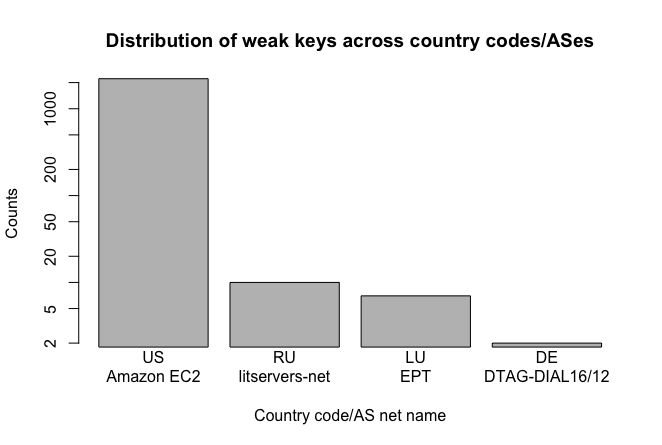
\includegraphics[width=\linewidth]{country-code-distribution.png}
\caption{Distribution of weak keys across country codes/ASes}
\label{country-code-distro}
\end{figure}


\begin{figure}[h]
\centering
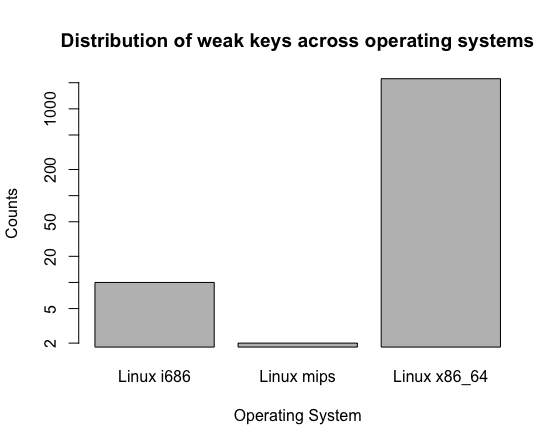
\includegraphics[width=\linewidth]{distribution-across-OS.png}
\caption{Distribution of weak keys across operating systems}
\label{dist-across-os}
\end{figure}


\begin{figure}[h]
\centering
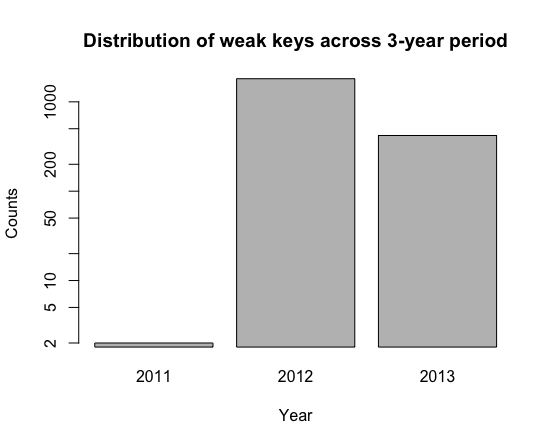
\includegraphics[width=\linewidth]{distribution-over-3-years.png}
\caption{Distribution of weak keys across 3-year period}
\label{dist-3-yrs}
\end{figure}

\begin{itemize}
    \item 2,217 of these 2,236 keys originated from Tor relay IP addresses with the US (United States) country code. Additionally, all of these originated from IP addresses with AMAZON-EC2 and AMAZON-ZIAD1 ASN net names.
    \item 10 of these 2,236 keys originated from Tor relay IP addresses with the RU (Russia) country code. Additionally, all of these originated from IP addresses with the litservers-net ASN net name. These Tor relays were published in November 2012.
    \item 7 of these 2,236 keys originated from Tor relay IP addresses with the LU (Luxembourg) country code. Additionally, all of these originated from IP addresses with the EPT ASN net name. These Tor relays were generated in November 2012. The authors~\cite{biryukov2013trawling} conducted their research at the University of Luxembourg.
    \item 2 of these 2,236 keys originated from Tor relay IP addresses with the DE (Germany) country code. Additionally, all of these originated from IP addresses with DTAG-DIAL16 and DTAG-DIAL12 ASN net names. These Tor relays were generated in late 2011.
\end{itemize}


\subsection{Signing keys with repeated moduli}
To my surprise, during my experiment, I found 10 Tor signing keys with repeated moduli. Their RSA public keys were distinct but their moduli were identical. I traced these keys to a 2014 attack against Tor's distributed hash table that's used for onion services.